\RequirePackage{luatex85,shellesc}
\documentclass[tikz, convert={outext=.svg, command=\unexpanded{pdf2svg \infile\space\outfile}}]{standalone}
\usepackage{luaotfload}
\usepackage{xcolor}
\usepackage{microtype}
\usepackage{fontspec}
\usepackage{unicode-math}
\definecolor{tableau1}{RGB}{78,121,167}
\definecolor{tableau1-light}{RGB}{155,198,244}
\definecolor{tableau2}{RGB}{242,142,43}
\definecolor{tableau3}{RGB}{225,87,89}
\UseMicrotypeSet[protrusion]{basicmath}
\defaultfontfeatures{Ligatures=TeX, Scale=MatchLowercase}
\setmainfont{Roboto}
\setmathfont{Libertinus Math}

\usetikzlibrary{calc}
\tikzset{
  axis/.style={
    dashed,
    -
  },
  reference/.style={
    dotted,
    thick,
    -
  },
  moment/.style={
    very thick,
    ->,
    >=stealth
  },
  disc-fill/.style = {
    draw=black,
    fill=tableau1-light
  },
}

\begin{document}
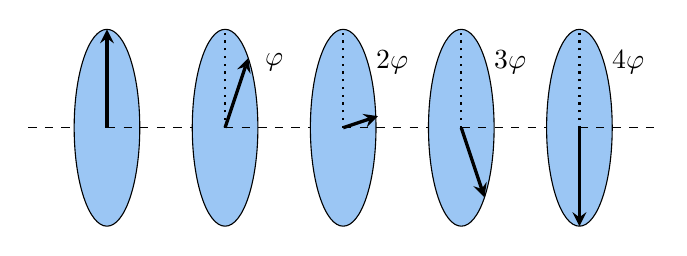
\begin{tikzpicture}

  \def\YSTART{3}
  \def\YDIAONE{2.5}
  \def\XONESTART{2}
  \def\XONEDELTA{1.5}

  \def\XONEEND{\XONESTART+\XONEDELTA}
  \def\XTWOSTART{\XONEEND+\XONEDELTA}
  \def\XTWOEND{\XTWOSTART+\XONEDELTA}
  \def\XTHREESTART{\XTWOEND+\XONEDELTA}
  \def\XTHREEEND{\XTHREESTART+1.0}
  \def\YONEMIDDLE{\YSTART+\YDIAONE/2}

  % discs
  \draw[axis] ($ (\XONESTART,\YONEMIDDLE)-(1,0) $) -- (\XONESTART, \YONEMIDDLE);
  
  \draw[disc-fill] (\XONESTART,\YONEMIDDLE) ellipse ({\YDIAONE/6} and {\YDIAONE/2});
  \draw[axis] (\XONESTART, \YONEMIDDLE) -- (\XONEEND, \YONEMIDDLE);
  
  \draw[disc-fill] (\XONEEND,\YONEMIDDLE) ellipse ({\YDIAONE/6} and {\YDIAONE/2});
  \draw[axis] (\XONEEND, \YONEMIDDLE) -- (\XTWOSTART, \YONEMIDDLE);
  
  \draw[disc-fill] (\XTWOSTART,\YONEMIDDLE) ellipse ({\YDIAONE/6} and {\YDIAONE/2});
  \draw[axis] (\XTWOSTART, \YONEMIDDLE) -- (\XTWOEND, \YONEMIDDLE);
  
  \draw[disc-fill] (\XTWOEND,\YONEMIDDLE) ellipse ({\YDIAONE/6} and {\YDIAONE/2});
  \draw[axis] (\XTWOEND, \YONEMIDDLE) -- (\XTHREESTART, \YONEMIDDLE);
  
  \draw[disc-fill] (\XTHREESTART,\YONEMIDDLE) ellipse ({\YDIAONE/6} and {\YDIAONE/2});
  \draw[axis] (\XTHREESTART,  \YONEMIDDLE) -- (\XTHREEEND, \YONEMIDDLE);
  
  % reference direction
  \draw[reference] (\XONESTART,  \YONEMIDDLE, 0) -- +(0, \YDIAONE/2, 0);
  \draw[reference] (\XONEEND,  \YONEMIDDLE, 0) -- +(0, \YDIAONE/2, 0);
  \draw[reference] (\XTWOSTART,  \YONEMIDDLE, 0) -- +(0, \YDIAONE/2, 0);
  \draw[reference] (\XTWOEND,  \YONEMIDDLE, 0) -- +(0, \YDIAONE/2, 0);
  \draw[reference] (\XTHREESTART,  \YONEMIDDLE, 0) -- +(0, \YDIAONE/2, 0);
  
  % moments
  \draw[moment] (\XONESTART,  \YONEMIDDLE, 0) -- +(0, \YDIAONE/2, 0);
  \draw[moment] (\XONEEND,  \YONEMIDDLE) -- +( ${1/sqrt(2)}*(\YDIAONE/6, \YDIAONE/2) $);
  \draw[moment] (\XTWOSTART,  \YONEMIDDLE) -- +($ {1/(2*sqrt(2))}*(\YDIAONE/2, \YDIAONE/6) $);
  \draw[moment] (\XTWOEND,  \YONEMIDDLE) -- +( ${1/(1*sqrt(2))}*(\YDIAONE/6, -\YDIAONE/2) $);
  \draw[moment] (\XTHREESTART,  \YONEMIDDLE) -- +(0, -\YDIAONE/2);
  
  % Angle labels
  \draw ($ (\XONEEND, \YONEMIDDLE) + (\YDIAONE/4, \YDIAONE/3) $) node {$\varphi$};
  \draw ($ (\XTWOSTART, \YONEMIDDLE) + (\YDIAONE/4, \YDIAONE/3) $) node {$2\varphi$};
  \draw ($ (\XTWOEND, \YONEMIDDLE) + (\YDIAONE/4, \YDIAONE/3) $) node {$3\varphi$};
  \draw ($ (\XTHREESTART, \YONEMIDDLE) + (\YDIAONE/4, \YDIAONE/3) $) node {$4\varphi$};
  
\end{tikzpicture}
\end{document}